%\section{Facility Location in Stable Instances}

In the previous section we saw that when we focus on the average instances of a problem, namely the "real-world" instances, we can avoid the hardness results and design better algorithms. Since clustering and facility location games are closely related problems, in this section we are going to see how perturbation stability in $k$-facility location games affects the design of mechanisms. Can we design strategyproof mechanisms with a bounded approximation ratio using the properties of stability? We have seen that in the simple setting where we want to locate $2$ facilities in the line any deterministic mechanism has $(n-1)$-approximation ratio because the agents have the power to change the clustering by misreporting their preferred location. So naturally it is very interesting to investigate the power any agent has in changing the structure of the clustering when the instance is stable and the clusters are well defined.


\section{Facility Location in Trees}


In this section, the agents are located in a Tree. With out loss of generality, we can view the tree with the location of agent $x_1$ as the root. We first need to adapt the definition of perturbation stability for the Facility Location games.

\begin{definition}[$\g$-Perturbation and $\g$-Stability]
Let $N$ be a set of $n$ agents located on a tree $(T,d)$, where $d$ is a metric distance function. Let $\x=(x_1,...,x_n)$ be a location profile. Let $\vec{z}= (z_1,...,z_m)$ denote the intersections on the tree, we will refer to them as phantom agents. A location profile $\xx=(x_1',...,x_n') \in (T,d')$ is a $\g$-perturbation of $\x$, for some $\g$, if for every pair of consecutive agents $x$ and $y$ (agents $x$ and $y$ can be any of $x_i-z_j$,$x_i-x_j$ or $z_i-z_j$ pairs) it holds:
\[ d'(x,y) \in  \bigg[\frac{1}{\g}d(x,y),d(x,y) \bigg]\]
 
A $k$-Facility Location instance $\x$, with optimal clustering $\CC=(c_1,...,c_k)$, is $\g$-(perturbation) stable, if for every $\g$-perturbation $\xx$ of $\x$ $\CC$ remains the unique optimal $k$-clustering.
\end{definition}


In order to properly define it we are going to assign phantom agents $\vec{z}=(z_1,...z_m)$ on every intersection of the tree. A $\g$-perturbation $\xx$ of an instance $\x$ can be obtained by scaling down any subset of pairs of consecutive agents, including the phantom agents, by a factor of at most $\g$. We can see that every valid metric-perturbation (Definition \ref{metricPer}) of the instance $\x$ (only agents' locations) can be performed by the process described above. Note that the distance between any pair of actual agents $x_i$ and $x_j$ is scaled down by a factor of at most $\g$ because the length of every pair of consecutive agents in the unique path that connects them is scaled down by a factor of at most $\g$. Moreover, the perturbed space is metric because the distance between $x_i$ and $x_j$ is the length of the unique shortest path between $x_i$ and $x_j$. Therefore, this class of $\g$-stable instances includes the class of $\g$-metric stable instances.  This notion of $\g$-perturbation captures all the perturbations that can be depicted on the same tree.

%We can perform every metric-perturbation but also perturbations that are not allowed by the definition for the clustering. For example we could scale down only the distance between an agent $x_i$ and a phantom agent $z_i$. 


\begin{figure}[ht]
    \centering
    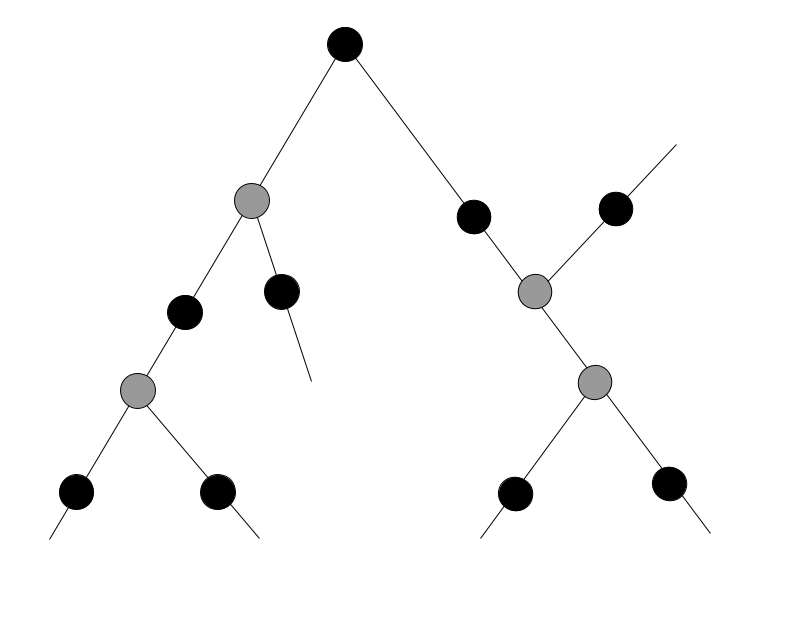
\includegraphics[width=8cm]{Images/Perturbation1.png}
    \caption{An example of a location profile $\x$ (black points) with phantom agents $\vec{z}$ on the intersections (gray points)}
    \label{fig:per}
\end{figure}



In the previous section, we showed that in general metric spaces in $\g$-stable instances, with $\g\ge2$, every cluster in the optimal solution forms a subtree in the minimum spanning tree. Similarly, we can show that this property holds when the underline metric space is a tree $T$. 
\begin{obs}\label{obs:subtrees}
Let $\x$ be a $\g$-stable, with $\g\ge2$, then in the optimal clustering $\CC$ every cluster $C_i$ forms a subtree.
\end{obs}

\begin{proof}
For contradiction suppose there exist a cluster $C_j$ that does not form a subtree, like in Figure \ref{fig:subtree}. Since the instance is stable we have that $d(x_{j_2},x_i)>(\g-1)d(x_{j_2},c_j)$. We also have that the distance between any two points is equal to the length of the unique path that connects those points, thus $d(x_{j_2},c_j) = d(x_{j2},x_i) + d(x_i,c_j)$. Using the previous inequality we get $d(x_{j_2},c_j)> (\g-1)d(x_{j2},c_j) + d(x_i,c_j) \implies d(x_i,c_j) < (2-\g) d(x_{j_2},c_j)$. When $\g\ge2$ the distance between $d(x_i,c_j)$ is negative but every distance function is non-negative.
\end{proof}

  
\begin{figure}[ht]
    \centering
    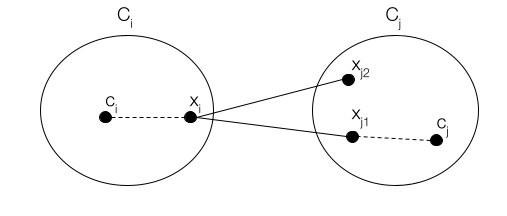
\includegraphics[width=10cm]{Images/FCStableTree.png}
    \caption{Example of a cluster that does not form a subtree.}
    \label{fig:subtree}
\end{figure}



As we mentioned before, perturbation stability implies that there is a structure in the original location profile. In other words, the optimal solution is resilient to minor changes. In the facility location setting, the agents are strategic, which means they are motivated to misreport in order to reduce their connection cost. The idea is to see how much power a strategic agent has to change the outcome of a mechanism with a single deviation now that the instance has a well-defined optimal solution. Let us point out that an agent's deviation is entirely different from a perturbation of an instance. An agent can misreport at any location in the metric space, which may result in a non-stable instance. However, after a perturbation, the distance between any two agents is at most $\g$ times smaller than in the original instance. 

%\subsection{The Optimal solution is strategyproof for $(2+\sqrt{3})$-stable instances}
\subsection{The Optimal solution is strategyproof for \texorpdfstring{$(2+\sqrt{3})$}-stable instances}



\begin{algorithm}[ht]
\label{algorithm:optimal}
\DontPrintSemicolon
\SetAlgoLined
\LinesNumbered
\KwResult{An allocation of $k$-facilities}
\KwIn{A $k$-Facility Location instance $\x$.}
Compute the optimal clustering
 $(C_1, \ldots, C_k)$. Let $c_i$ be the median point of each cluster $C_i$.\;

 \uIf{\big($\exists i \in [k]$ with $|C_i|=1$\big) or \big($\exists \;x_i,x_i'\in Ci$ and  $x_j,x_j'\in C_j$ with $\max\{ d(x_i,x_i'), d(x_j,x_j')\} \geq d(x_i,x_j) $\big)}{
 \KwOut {``FACILITIES ARE NOT ALLOCATED''.}}\uElse{
 
\KwOut {The $k$-facility allocation $(c_1, \ldots, c_k)$ \;}}

\caption{\textsc{Optimal}}
\end{algorithm}

We next show that the the mechanism that returns the optimal solution is strategyproof for $(2+\sqrt{3})$-stable instances whose optimal clustering does not include singleton clusters. We need to exclude the stable instances with singleton clusters in their optimal solution from the mechanism because there is always an agent that can benefit by becoming a singleton cluster. Consider a $\g$-stable instance $\x$. Suppose an agent $x_i \in C_i$ reports a location $x'$ far away from any location in $\x$ creating a different instance $\x\,'$. Since the mechanism allocates the facilities optimally $x'$ becomes a singleton cluster. Now the mechanism has to allocate $k-1$ facilities to the remaining agents, which means two clusters from the original optimal solution merge. We can always create an instance in which cluster $C_i$ merges with its neighbor cluster $C_j$ which makes the new median closer to $x_i$. The main problem is that the new instance $\x\,'$ is also $\g$-stable as the original and there is no way to determine whether or not there is a deviation. 


\begin{figure}[ht]
    \centering
    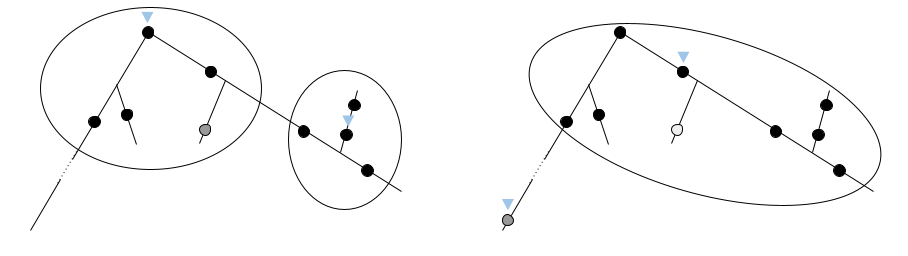
\includegraphics[width=\textwidth]{Images/singleton.png}
    \caption{Singleton Deviation}
    \label{fig:singleton}
\end{figure}

It is also important to remember that we cannot efficiently estimate the stability factor of a given instance. This is why we rely on the properties that derive from stability, since the properties are necessary but not sufficient for stability. That also means that the mechanism serves instances that are non-stable but satisfy the cluster separation property. We can efficiently check if the cluster separation property is violated between any to clusters. Since every cluster in the optimal solution forms a subtree, we only have to check if any of the $k-1$ edges between 2 different clusters violates the cluster separation property.


\begin{theorem}
The \textsc{Optimal} Mechanism applied to $(2+\sqrt{3})$-stable instances of $k$-Facility Location without singleton cluster in their optimal clustering is strategyproof and minimizes the social cost. 
\end{theorem}


%proof optimal
\begin{proof}
The mechanism returns the optimal solution, so we only need to prove that it is strategyproof. Let any $(2+\sqrt{3})$-stable instance with optimal clustering $\CC = (C_1,..., C_k)$. Suppose agent $x_i \in C_i$ reports a location $y$ in order to decrease her cost. Let $\y = (\x_{-i},y)$ be the instance after the deviation, and $\Y$ be its optimal clustering.There are three possible deviations:
\begin{enumerate}[1.]
    \item If $y$ is in the area of $C_i$, then the clustering structure would not change. But the median location for one facility on trees is strategyproof and thus she cannot benefit from such deviation.
    \item If $y$ is a singleton cluster in $\Y$, then the mechanism would not allocate any facilities, making her cost infinite times larger.
    \item If $y$ is cluster together with agents from different clusters in $\CC$. 
\end{enumerate}

We will only focus on the third case since this is the only way she could benefit. In order for the mechanism to be strategyproof, we need to show that either the deviation is not profitable ($d(x_i,\CC) < d(x_i,\Y)$) or that the cluster separation property is violated and no facilities are allocated. 

We have that $y$ is clustered together with agents belonging in one or two clusters of $\CC$, let that clusters be $C_j$ and $C_l$. In $\Y$ the number of facilities serving agents from $C_j\cup C_l \cup \{y \}$ are at least the number of facilities serving agents from $C_j\cup C_l$ in $\CC$, because both $\CC$ and $\Y$ are optimal clusterings. Suppose one facility is placed to an agent in $C_j$. The original instance is $2+\sqrt{3}$-stable, so by the separation property we have that every agent is closer to every agent from her own cluster that to any other agent from a different cluster. This implies that no agent in $C_j$ is served by a facility in $\x\setminus C_j$. 
 
\begin{description}
\item[Case 1:] \textit{ $y$ is not allocated a facility in $\Y$}: This can happen in one of two ways:
    \begin{description}
        \item[Case 1a:] $y$ is clustered together with some agents from cluster $C_j$ and no facility placed in $C_j$ serves agents in $\x\setminus C_j$ in $\Y$. 
        
        \item[Case 1b:] $y$ is clustered together with some agents from a cluster $C_j$ and at least one of the facilities placed in $C_j$ serve agents in $\x\setminus C_j$ in $\Y$.
\end{description}
        
\item[Case 2:] \textit{$y$ is allocated a facility in $\Y$}. This can happen in one of two ways:

 \begin{description}
        \item[Case 2a:] $y$ only serves agents that belong in $C_j$ (by optimality, $y$ must be the median location of the new cluster, which implies that either $y$ is not in the area of $C_j$ and only serves one agent from $C_l$ or $y$ is in the area of $C_j$ and serves multiple agents).
        \item[Case 2b:] In $\Y$, $y$ serves agents that belong in both $C_{j-1}$ and $C_j$.
\end{description}
\end{description}

We first consider the cases 1a and 2a, namely the cases where in $\Y$ there is a facility in $C_j$ that only serves agents in $C_j$. If there is only one facility allocated in $C_j\cup\{y\}$ then both clusterings $\CC$ and $\Y$ have the same structure, making $x_i$'s deviation not profitable. So, in $\Y$ there must be two facilities in $C_j\cup\{y\}$. Suppose there is a location $y$ such that the deviation is profitable, $d(x_i,\CC) > d(x_i,\Y)$. Since $\Y$ is the optimal clustering for $\y$ we have that:
\begin{align*}
    cost(\y,\CC) &> cost(\y,\Y) \iff \\
    cost(\x,\CC) + d(y,\CC) - d(x_i,\CC) &> cost(\x,\Y) + d(y,\Y) - d(x_i,\Y) \iff \\
    d(y,\CC) - d(y,\Y) &> cost(\x,\Y) - cost(\x,\CC)  + d(x_i,\CC) - d(x_i,\Y)
\end{align*}

Since $i$'s deviation to $y$ is profitable ($d(x_i,\CC) - d(x_i,\Y)>0$) we get:

\begin{align}
\begin{split}
d(y,\CC) - d(y,\Y) &> cost(\x,\Y) - cost(\x,\CC)\label{eq:gainy} \\
&= cost(C_j,\Y)-cost(C_j,\CC)-cost(\x\setminus C_j,\Y)-cost(\x\setminus C_j,\CC)
\end{split}
\end{align}


    
%{???}

We now consider a valid $\gamma$-perturbation $\xx$ of the original instance $\x$: We first remove from the instance all the agents from $C_j$ and all the edges connected to them. This may break the instance in more than one connected components. By observation \ref{obs:subtrees}, we have that there is no cluster whose agents belong in more than one connected components. Then, we scale down by $\g$ all the distances between consecutive agents that are in the same connected component. By stability, the clustering $\CC$ remains the unique optimal clustering for $\xx$ therefore $cost(\xx,\CC) < cost(\xx,\Y)$. Since, in cases 1a and 2a, the facility allocated to an agent of $C_j\cup \{y\}$ does not serve agents in $\x \setminus C_j$ in $\CC$ and $\Y$ we have:
\begin{align*}
 cost(\xx, \CC) = cost(C_j,\CC)+\frac{1}{\gamma}cost(\x\setminus C_j,\CC)\\
 cost(\xx, \Y) = cost(C_j,\Y)+\frac{1}{\gamma} cost(\x\setminus C_j,\Y)
\end{align*}
Using that $cost(\xx,\CC) < cost(\xx,\Y)$ and  that for any $\gamma\ge2$ it holds $\frac{1}{\gamma} \le 1-\frac{1}{\gamma} $ we get:
\begin{align}
   cost(C_j,\CC) - cost(C_j,\Y) &< \frac{1}{\gamma} \left( cost(\x\setminus C_j,\Y) - cost(\x\setminus C_j,\CC) \right)\label{eq:costIneq1} \\
    &\le (1 -\frac{1}{\gamma}) \left( cost(\x\setminus C_j,\Y) - cost(\x\setminus C_j,\CC) \right) \label{eq:costIneq}
\end{align}

Rearranging (\ref{eq:costIneq}) we get:
\begin{equation}
    cost(\x,\Y) - cost(\x,\CC) > \frac{1}{\gamma}\left( cost(\x\setminus C_j,\Y) - cost(\x\setminus C_j,\CC) \right)\label{eq:lowerBcostY}
\end{equation}

%{?????????????}
 
%To prove the previous inequality it suffice to show that the decrease in the cost of $y$ due to the additional facility in $\Y$ is at most the decrease in the cost of an agent from $C_j$ in $\Y$.
We know that there are at least two facilities serving $C_j\cup\{y\}$. Let $Y_{j_1}$ be the cluster that contains $y$ and some agents of $C_j$. In case 1a, let $x_j \in Y_{j_1}$ be the agent that has the facility. Then the decrease in the cost of $y$ due to the additional facility in $\Y$ is at most the decrease in the cost of an agent from $C_j$ in $\Y$. In case 2a, where agent $y$ has a facility, by optimally of $\Y$, we have that $y$ is the median of the new cluster. If we view $c_j$ as the root of the tree then $y$ has at least one agent from $C_j$ as a child; otherwise it would not be the median location. Therefore, the decrease in the cost of $y$ is at most the decrease in the cost of an agent from $C_j$ in $\Y$. (The case where $y$ is not in the area of $C_j$ and only serves one agent is equivalent to placing the facility on the other agent and serving $y$ from there). In both cases, we can bound from below the total decrease in the cost of $C_j$ due to the additional facility.

\begin{align*}
   d(y,\CC)-d(y,\Y)  &\le cost(C_j,\CC)-cost(C_j,\Y) \xRightarrow{(\ref{eq:costIneq1})}\\
   &\le \frac{1}{\gamma} \left( cost(\x\setminus C_j,\Y) - cost(\x\setminus C_j,\CC) \right) \xRightarrow{(\ref{eq:lowerBcostY})}\\
   &< cost(\x,\Y) - cost(\x,\CC)
\end{align*}

Which contradicts equation (\ref{eq:gainy}).


%---------------------------------------------------------------------------------------------

\bigskip

Now we consider cases 1b and 2b, namely the cases where some agents of $C_j$ are clustered with agents of $C_l$. Let $Y_{j_1}$ and $Y_{j_2}$ denote the clusters of $\Y$ that include all the agents of $C_j$. Let $Y_{j_1}$ be the cluster that has agents from $C_j$ and $C_l$. Consider $x_1 \in Y_{j_1} \cap C_j$, $z\in Y_{j_1} \cap C_l$ and $x_2 \in Y_{j_2}\cap C_j$. By the cluster separation property $d(x_1,z) \ge D_{x_1}$, where $D_{x_1}$ is the largest intra-cluster distance from $x_1$. Since $x_1$ and $x_2$ belong in the same cluster in $\CC$ we have that $d(x_1,x_2)<D_{x_1}$. Therefore, $d(x_1,z)>d(x_1,x_2)$ which violates the cluster separation property, since an intra-cluster distance is greater than an inter-cluster distance. In this case, the mechanism will not allocate any facilities. 
\end{proof}


\iffalse
\section{Lower bound on stability }




\begin{theorem}
For every $k\ge3$ and $\delta>0$, any deterministic anonymous strategy proof mechanism for $(\sqrt{2}-\delta)$-stable instances of $k$-facility location on the line with $n\ge k+1$ agents has an unbounded approximation ratio.
\end{theorem}
\fi
%----------------------------------------------------------------------------------------------

%\section{General metrics}
%\subsection{The \textsc{Random} mechanism is strategyproof for 5-Stable instances}

%\begin{theorem}

\end{theorem}

\begin{proof}
Let $\vec{x}$ be any $5-$stable instance with optimal clustering $\vec{C} = (C_1,...,C_k)$. Let $\vec{x}' = (\vec{x}_{-i},x')$ be the resulting instance after agent $i$ deviates from location $x_i$ to $x'$, with optimal clustering $\vec{C'}$. In the original clustering $x_i\in C_i$. Since the mechanism places a facility at a location of an agent selected uniformly at random from each optimal cluster, no agent can gain by deviating within the range of her optimal cluster. Therefore we need to cover all $i$'s possible deviations that result in a different clustering than the original. This can happen in three ways:

\begin{itemize}
\setlength\itemsep{0.1em}
  \item[]\textbf{Case 1:} Becoming a member of another cluster
  \item[]\textbf{Case 2:} Becoming a self serving cluster
  \item[]\textbf{Case 3:} Merging or splitting $C_i$
\end{itemize}


In case 1, agent $i$ is clustered together with members from a different cluster in $\vec{C}$ without splitting or merging $C_i$. The deviation from $x_i$ to $x'$ results in either an increase in her expected cost or a violation of the cluster separation property in $\vec{C}'$.


First, we need to compute the expected $i$'s cost if she reports her true location. We can define as $X_i$ the discrete random variable that takes values from the sample space $\{ d(x,x_i): x\in C_i\}$ uniformly at random. Let $|C_i|=n$. Then, her expected cost is:

\[ E[X_i] = \frac{\sum_{x\in C_i} d(x,x_i)}{n} \]

Note that $i$'s cost is at most $D(C_i)$ since the center is selected uniformly at random among the agents in $C_i$.



In this case, agents in $C_i$ are not merged or splitted in $\vec{C}'$. So, all the agents that were originally cluster together with $x_i$ in $\vec{C}$ are cluster together in $\vec{C}'$. Let that be $C_i'$. %($x\in C_i\setminus x_i$) 
%needs haaalp!!
Let $C_j'$ be the cluster that $x_i$ belongs in $\vec{C}'$. Since she is trying to make the deviation profitable $C_j'$ need to be the closest cluster, different from $C_i'$, to her original location.


After this change in the clustering we need to compute $i$
's expected cost. Same as before, we can define as $X_i'$ the discrete random variable that takes values from the sample space $\{ d(x,x_i): x\in C_i' \}  \equiv \{ d(x,x_i): x\in C_i, x\neq x_i \}$ and $X_j'$ the discrete random variable that takes values from the sample space $\{d(x',x_i)\} \	\cup \{ d(x,x_i): x\in C_j'\}$ uniformly at random. $X_i'$ represents $i$'s cost if she is served by the facility placed in $C_i'$ and $X_j'$ her cost if she is served by the facility in $C_j'$. Her expected cost becomes $\mathbb{E} [min\{ X_i', X_j' \}]$, since she can choose the facility closest to $x_i$. 
By the cluster separation property for any agent $x_j \notin C_i$ it holds that $d(x_i,x_j)>D(C_i)$.  We know that: 
\[\mathbb{E}[X_j'] =  \frac{\sum_{x \in C_j'} d(x,x_i) + d(x',x_i)}{|C_j'|+1}\]

If $d(x_i,x') > D(C_i)$ then all the values from $X_j'$'s sample space are larger than  $X_i$'s. Thus, agent i will always has small expected cost if she chooses the facility placed in $C_i'$. 
\[\mathbb{E}[min\{X_i',X_j'\}] = \mathbb{E}[X_i'] = \frac{\sum_{x \in C_i'} d(x,x_i)}{n-1} = \frac{\sum_{x \neq x_i\in C_i} d(x,x_i)}{n-1} > \mathbb{E}[X_i]\]

Since she is not a member of $C_i'$ she cannot affect the facility's location, making her expected cost higher than her original expected cost.
\bigskip

The only way she can gain by the deviation is if $x'$ belongs in $C_j$ and $d(x',x_i)<D(C_i)$. This way, she is close enough to her original location to make the deviation profitable but far enough to change the original clustering. Consider the case where $c_i$, $x_i$ and $x_j$ are collinear, $x_j$ being the agent from $C_j$ closest to $x_i$. In any other case, the distance $d(x',C_i')$ will be smaller, making the deviation easier to detect. 

By the cluster separation property for the stability factor of $5$, we have that  $d(x_i,x_j) = d(C_i,C_j) \ge 1.6\cdot D(C_i)$. In order for this distance to be tight all it must be $d(x_i,c_i) = 0.4D(C_i)$. We also have that $d(x_j,c_j) < 0.4D(C_i)$, since by stability it holds $d(x_i,x_j) > (\gamma-1)d(x_j,c_j)$. Combining the above inequalities and that $d(x',x_i)<D(C_i)$ we get:
\begin{align}
d(x',c_i) \le d(x',x_i) + d(x_i,c_i) \le 1.4D(C_i) \\
d(x',x_j)>d(x_i,x_j) - d(x_i,x') > 0.6D(C_i)
\end{align}


Finally we need to distinguish two cases regarding the cluster $C_j'$: 
\begin{enumerate}
    \item $c_j \in C_j'$:  We have that $D(C_j') \ge d(c_j,x')$ and that $d(C_i',C_j') \le d(c_i,x') \le 1.4 D(C_i)$. By stability it hold $d(x_i,c_j) > \gamma d(x_i,c_i) = 2D(C_i)$. From triangle inequality it holds $d(c_j,x') \ge  d(c_j,x_i)-d(x_i,x') > D(C_i)$. Therefore, we get that $d(C_i',C_j') \le 1.4 D(C_i) < 1.4 D(C_i')$ 
    
    \item $c_j \notin C_j'$: In this case the agents from $C_j$ are splitted in (at least) two clusters in $\vec{C}'$. Let $C_l'$ be the cluster than $c_j$ belongs to. Since $x_j\in C_j'$ and $c_j \in C_l'$ we have that $d(C_j',C_l') \le d(c_j,x_j) < 0.4D(C_i)$. But $D(C_j') \ge d(x_j,x')>0.6D(C_i)$. Combining this inequalities we get $D(C_j',C_l') \le 0.67 D(C_j')$ which violates the minimum distance between  $C_j'$ \& $C_l'$.
\end{enumerate}

\end{proof}




\section{Conclusion and Future Work}
Remember that without making any assumptions about the instance, we cannot design strategyproof mechanisms with a bounded approximation because we cannot identify the optimal clusters in a strategyproof way. However, if we focus on perturbation stable instances, the structure helps us avoid that problem. Now we can efficiently find the optimal solution and place the facilities within each optimal cluster. We also showed that the strategic agents do not have the power to change the structure of the instance for a stability factor $\g\ge2+\sqrt{3}$ because all the inter-cluster distances are greater than the intra-cluster distances. This allows us to reduce the multi-facility location games on stable instances to a one-facility location game and use all the known results.

In the \textsc{Optimal} mechanism, we saw that we have to exclude the instances that contain singleton clusters because an agent can deviate to a location far away and bring a facility closer to her true location (singleton deviation). One way to overcome this problem is to limit the range of possible locations each player can declare based on their actual locations. In this case, we must also see how stable the instance must be in order for the optimal solution to be strategyproof.

Another direction is to assume a ``weaker" notion of stability in the instances. In the literature, $(\g,\epsilon)$-perturbation stability was also proposed, which states that at most $\epsilon n$ total points can swap into or out of each cluster under any $\g$ perturbation. These instances are more likely to describe ``real world"  instances. However, the non-stable points may be harder to handle.







